\documentclass[pdftex,11pt,letter]{article}
\usepackage{appendix} %http://www.tex.ac.uk/cgi-bin/texfaq2html?label=appendix
\usepackage{cancel}
\usepackage{amsmath,amssymb,latexsym,float,epsfig}
\usepackage{framed,color,url,fancybox,fullpage,booktabs,subfigure,wrapfig,chngpage,setspace}

\usepackage{amsfonts,caption}
\usepackage{hyperref}
\usepackage{graphicx}
\usepackage{color,epsfig}
\usepackage{bm}
\usepackage{enumerate}
\usepackage{amsmath, amssymb, graphics, setspace,mathtools}
\usepackage{float}
\usepackage[section]{placeins} % places floats within the section
\usepackage[superscript]{cite}


\newcommand{\ssection}[1]{\section[#1]{\centering\normalfont\scshape #1}}
\newcommand{\ssubsection}[1]{\subsection[#1]{\raggedright\normalfont\itshape #1}}
\newcommand\norm[1]{\left\lVert#1 \right\rVert}
\newcommand{\e}{\mathrm{e}}
\newcommand{\pderiv}[2]{\frac{\partial #1}{\partial #2}}
\numberwithin{equation}{section}
\numberwithin{figure}{section}
\usepackage{epstopdf,fancyvrb,cite,hyperref,jvlisting}
%\usepackage[options]{mcode}

\usepackage{pdflscape}%http://texblog.org/2007/11/10/landscape-in-latex/

\newcommand{\ul}[1]{\underline #1}

% Define commands 
\newcommand{\half}{\ensuremath{\frac{1}{2}}}
\newcommand{\bea}{\begin{eqnarray}}
\newcommand{\eea}{\end{eqnarray}}
\newcommand{\beq}{\begin{equation}}
\newcommand{\eeq}{\end{equation}}
\newcommand{\bdm}{\begin{displaymath}}
\newcommand{\edm}{\end{displaymath}}

\newcommand{\etal}[0]{{\em et al.}}
\newcommand{\etc}[0]{{\em etc.}}
\newcommand{\ie}[0]{{\em i.e.,}}


\newcommand{\pd}[2]{\dfrac{\partial #1}{\partial #2}}
\newcommand{\pf}[2]{\dfrac{d #1}{d #2}}
\newcommand{\pdt}[2]{\dfrac{\partial^2 #1}{\partial #2^2}}
\newcommand{\pft}[2]{\dfrac{d^2 #1}{d #2^2}}
\newcommand{\pdtno}[2]{\dfrac{\partial^2 #1}{\partial #2}}
\newcommand{\pdd}[3]{\dfrac{\partial^2 #1}{\partial #2 \partial #3}}
\newcommand{\pff}[3]{\dfrac{d^2 #1}{d #2 d #3}}


\renewcommand\floatpagefraction{0.99}
\renewcommand\topfraction{0.99}
\renewcommand\bottomfraction{0.99}
\renewcommand\textfraction{0.0}

\usepackage{titling}
\setlength{\droptitle}{-1in}   % This is your set screw

% For \url{SOME_URL}, links SOME_URL to the url SOME_URL
\providecommand*\url[1]{\href{#1}{#1}}
% Same as above, but pretty-prints SOME_URL in teletype fixed-width font
\renewcommand*\url[1]{\href{#1}{\texttt{#1}}}

% For \email{ADDRESS}, links ADDRESS to the url mailto:ADDRESS
\providecommand*\email[1]{\href{mailto:#1}{#1}}

\usepackage[superscript]{cite}
\usepackage{tikz}
%\begin{figure}
% \centering 
% 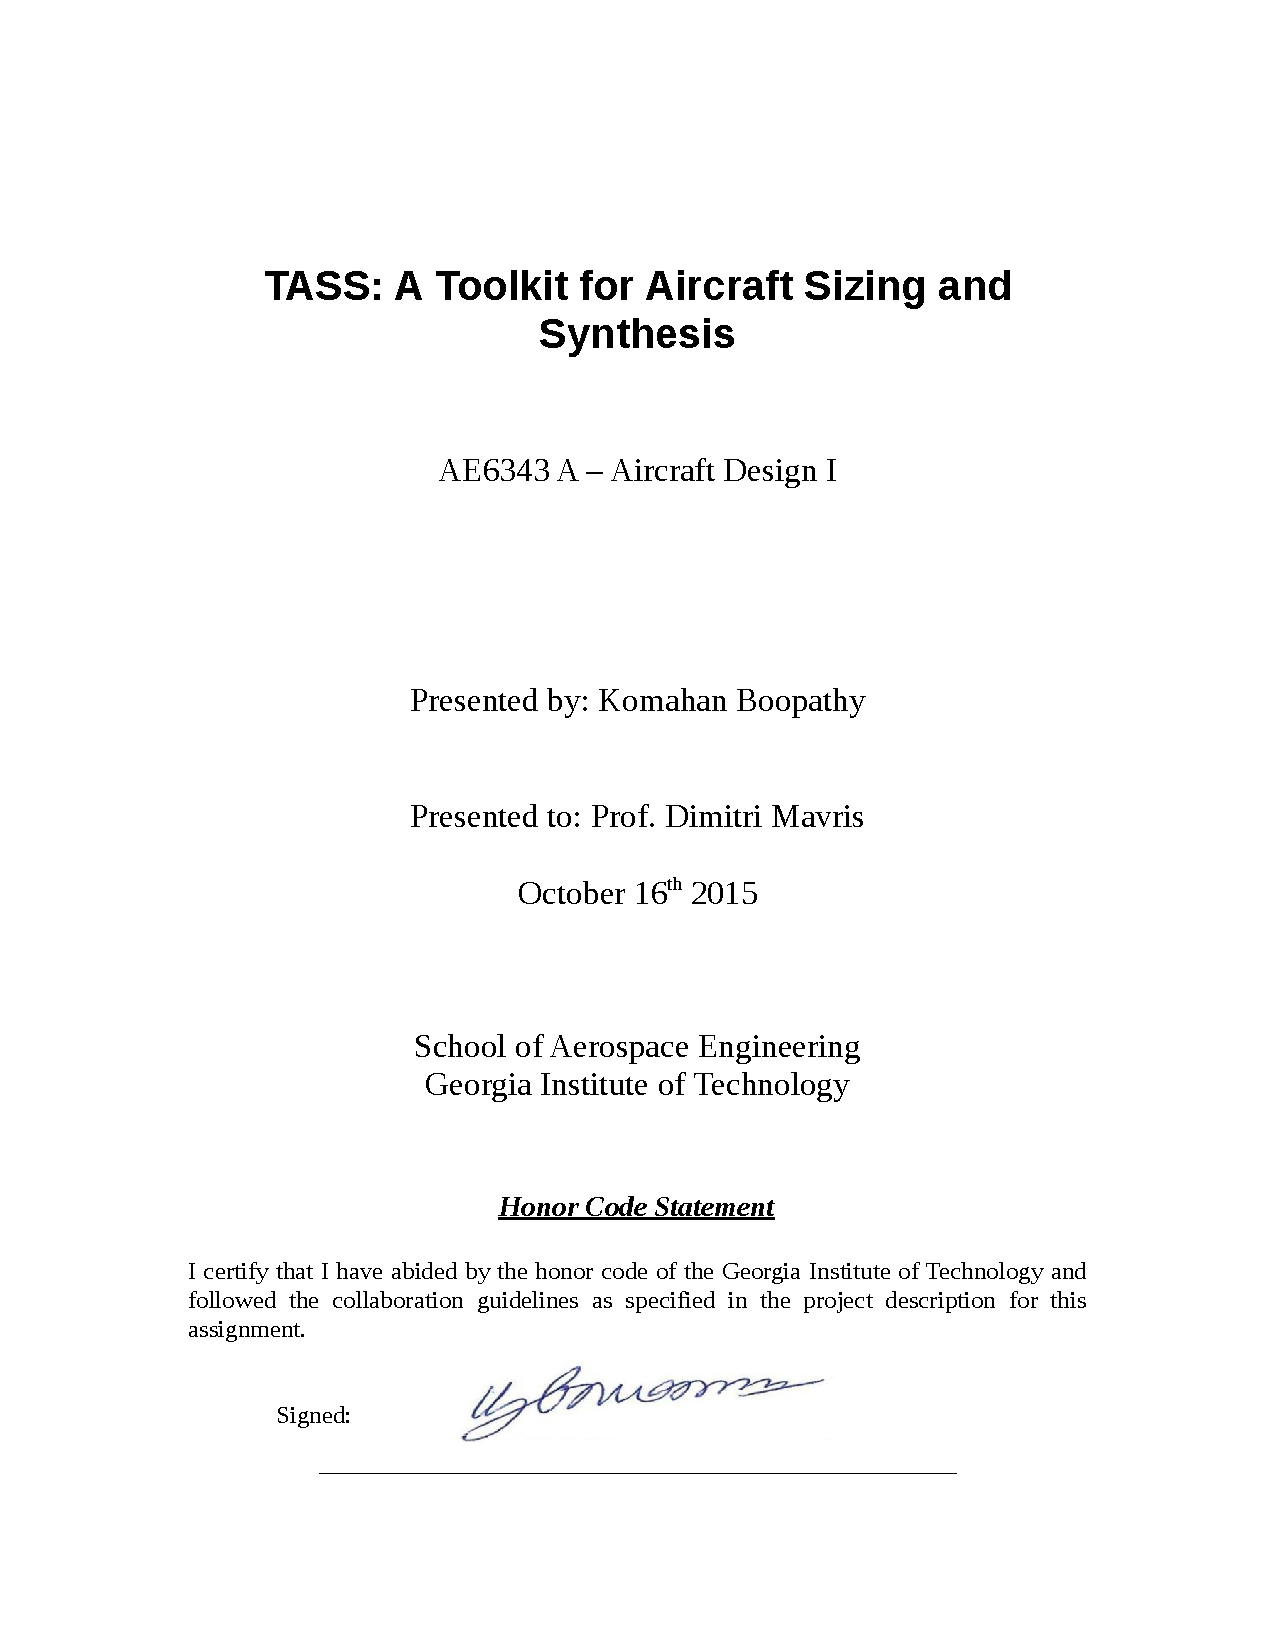
\includegraphics{Cover.pdf}
%\end{figure}




\title{\textbf{\textsc{TASS}: A Toolkit for Aircraft Sizing and Synthesis}}
\author{Komahan Boopathy~~\url{komahan@gatech.edu}} \date{\today}
\begin{document}
 \begin{tikzpicture}[remember picture,overlay]
    \node[inner sep=0pt] at (current page.center) {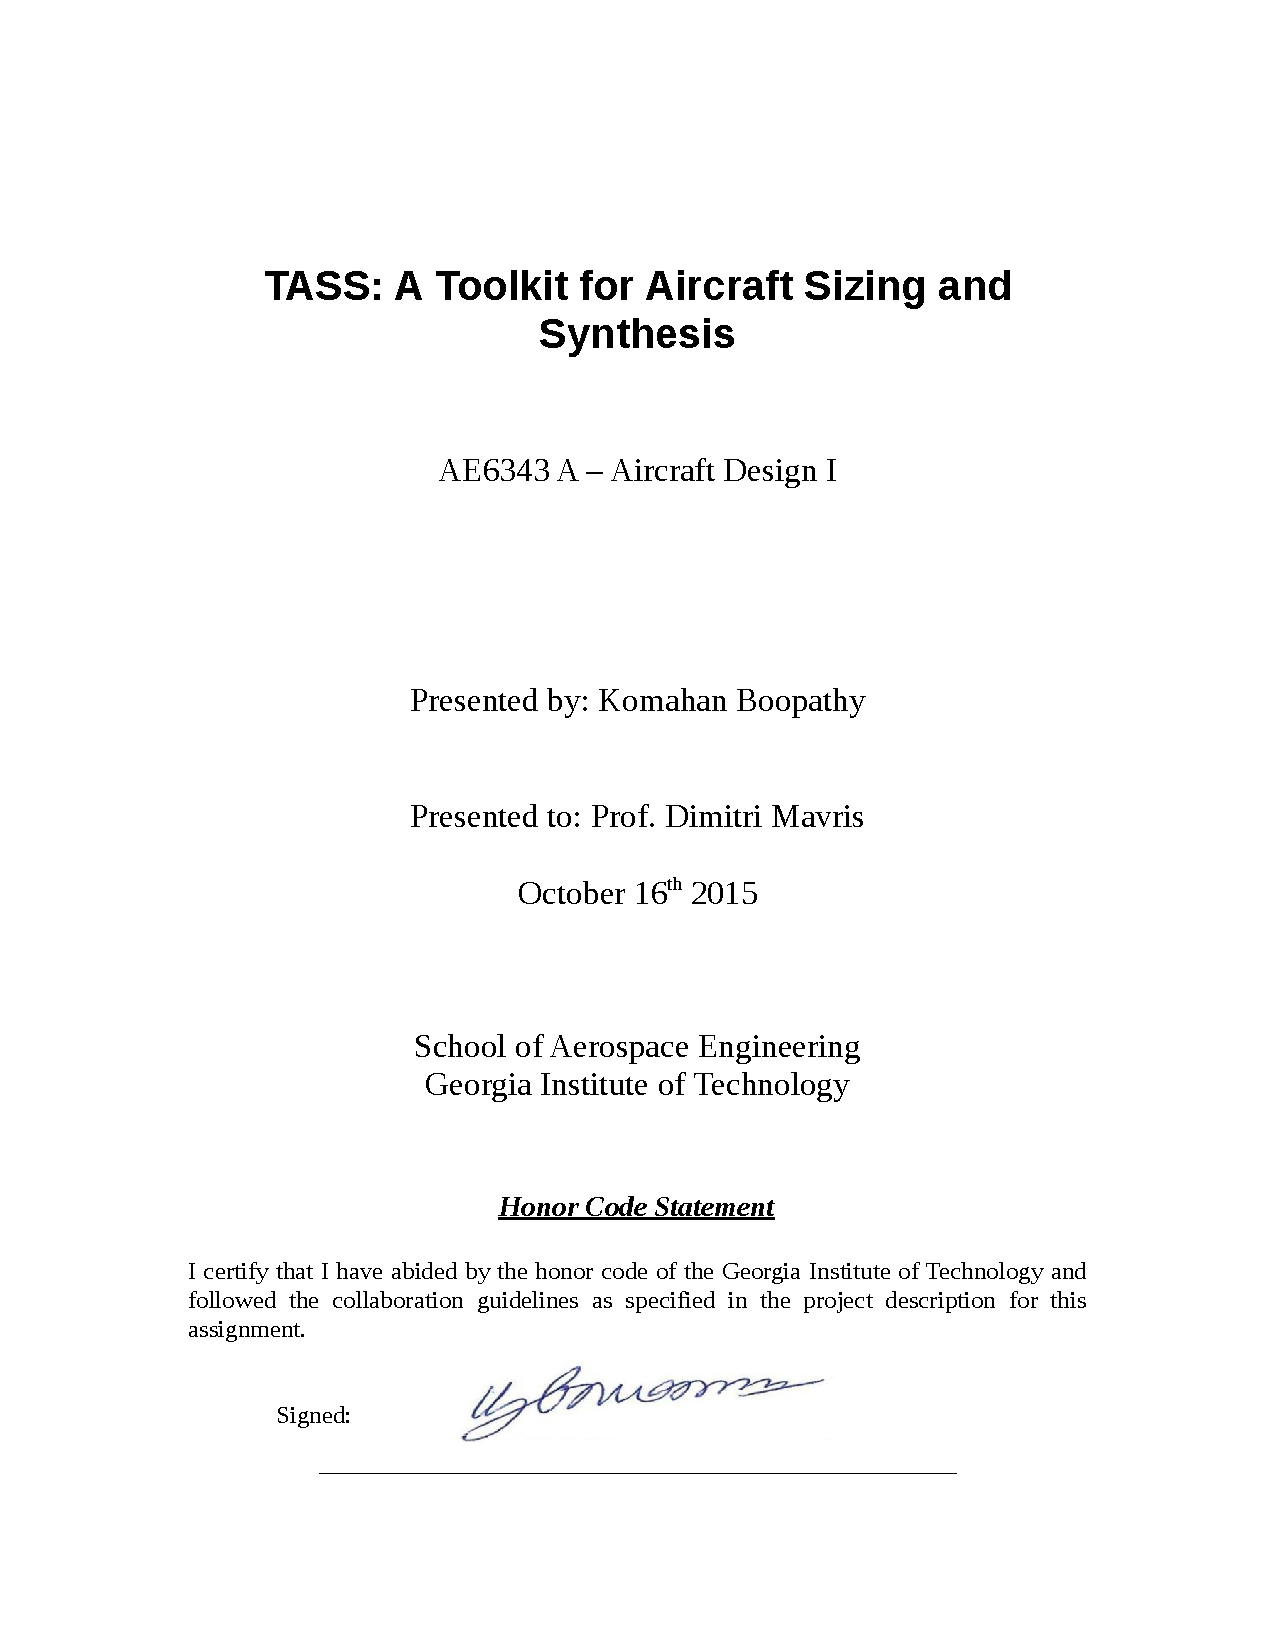
\includegraphics[page=1]{Cover.pdf}};
  \end{tikzpicture}

\clearpage
\tableofcontents
\clearpage
\listoffigures
\listoftables

\maketitle
\vspace{-0.25in}
\rule{\linewidth}{2pt}

\begin{abstract}
A  \ul{T}oolkit for \ul{A}ircraft \ul{S}izing and \ul{S}ynthesis (TASS), capable of performing sizing and synthesis calculations  in the context of conceptual design of aircraft is developed in Matlab\cite{MATLAB}. The TASS implements energy-based constraint and weight-fraction approach for the mission sizing analyses, and provides the user with a design point that is a function of \emph{thrust-weight ratio} and \emph{wing-loading}.  The performance of the TASS is benchmarked against the known metrics of a transonic jet fighter aircraft F-86 Sabre (Sabrejet).
\end{abstract}

\section{Introduction and Motivation}

Design of aircraft is subject to tens of thousands of constraints that span across a variety of disciplines such as aerodynamics, structures, controls and performance\cite{NicolaiText,FieldingText,HoweText,RaymerText}. Examples of such constraints, to name a few are: achieving a long cruise range, minimizing the take-off distance, fuel-efficient engines, stealth capabilities for reconnaissance, lift-constrained-drag-minimization, stress and strain requirements, and so on. These constraints are indeed the ones that drive the design and play a pivotal role in shaping the end-design. There has been an increased interest in exploring more at initial stages of design to identify conventional as well as non-conventional configurations -- a strategy that helps one to get a better insight of potential configurations that can meet the design requirements and eliminate retrospective changes that may be due at later stages of the design process, that are known to be prohibitively expensive. 
\\\\
Similar motivations have led to development of tools that ably perform conceptual analysis in various platforms\cite{Raymer2004, Kroo2005}. To this end, this work too aims to develop a toolkit in Matlab\cite{MATLAB} known as TASS, that performs an analysis of the early phases of aircraft design \ie~the sizing and synthesis. The scope of current work is limited to the conceptual design phase of aircraft design; more advanced phases in aircraft design (e.g. preliminary, detailed design \etc) fall beyond the scope of current work. Nevertheless, modularity is a key consideration in the development of the toolkit, which enables further advancements a function of time.
\\\\
Energy based constraint analyses encompass an attractive way to start with aircraft design. The main advantage of energy-based approach over conventional approaches is that it employs Lagrangian paradigm of mechanics, as opposed to Newton's world of vector mechanics. The key idea is that aircraft is treated as a system that converts energy from one form to another as the mission progresses. For example, combustion in the engines convert the chemical energy of the fuel into thermal energy, which in-turn accelerates the gases to rotate the turbines to provide mechanical energy to sustain motion. It is easier to think in terms of scalars such as potential energy (depends on position) and  kinetic energy (depends on rate of change of position), compared to resolving forces (e.g. lift, thrust)  along different directions (e.g. vertical, horizontal) and invoking force and moment balances. Due to such advantages, the \textsc{TASS} preferably employs energy based constraint analyses. The mathematical and physical models used in various stages of the mission are explained as and when they are introduced in later sections and are not explained here for brevity.

\section{Installation and Working }\label{layout}
This section is devoted to provide a high-level overview of the of the software. A Graphical User Interface (GUI) is designed to collect all the mission-specific inputs that the user supplies to the software. From an user-standpoint these input parameters are decided based on the complete break-down of mission requirements (e.g. humanitarian, rescue, military missions). 

\subsection{Installation}
The TASS uses native Matlab code for all of its functionality -- including initialization, iterative calculations and graphics, therefore a working version of Matlab\cite{MATLAB} is sufficient. The software is tested to work on both UNIX and Windows based workstations. The source code can be obtained by using \texttt{git clone https://github.com/komahanb/tass.git} from a \textit{terminal} or \textit{shell} program or by downloading \texttt{tass.zip} file and extracting it in a working folder of convenience. 

%Table~\ref{inputs} presents the typical inputs that the user is expected to provide to the software. 

\subsection{Constraint Analysis Layout}
The constraint analysis layout is designed to take a large number of input parameters. This, indeed increases the complexity of use but makes the tool more robust in terms of accommodating wide array of inputs and helps the user to analyze more flight conditions.  Figure~\ref{constraints_layout} shows the layout designed for the constraint analyses.
\paragraph{Execution:}
The user can run this layout by typing \texttt{constraint\_analysis} in MATLAB command line or by opening \texttt{constraint\_analysis.fig} file.
\begin{figure}[h!]
	\centering
	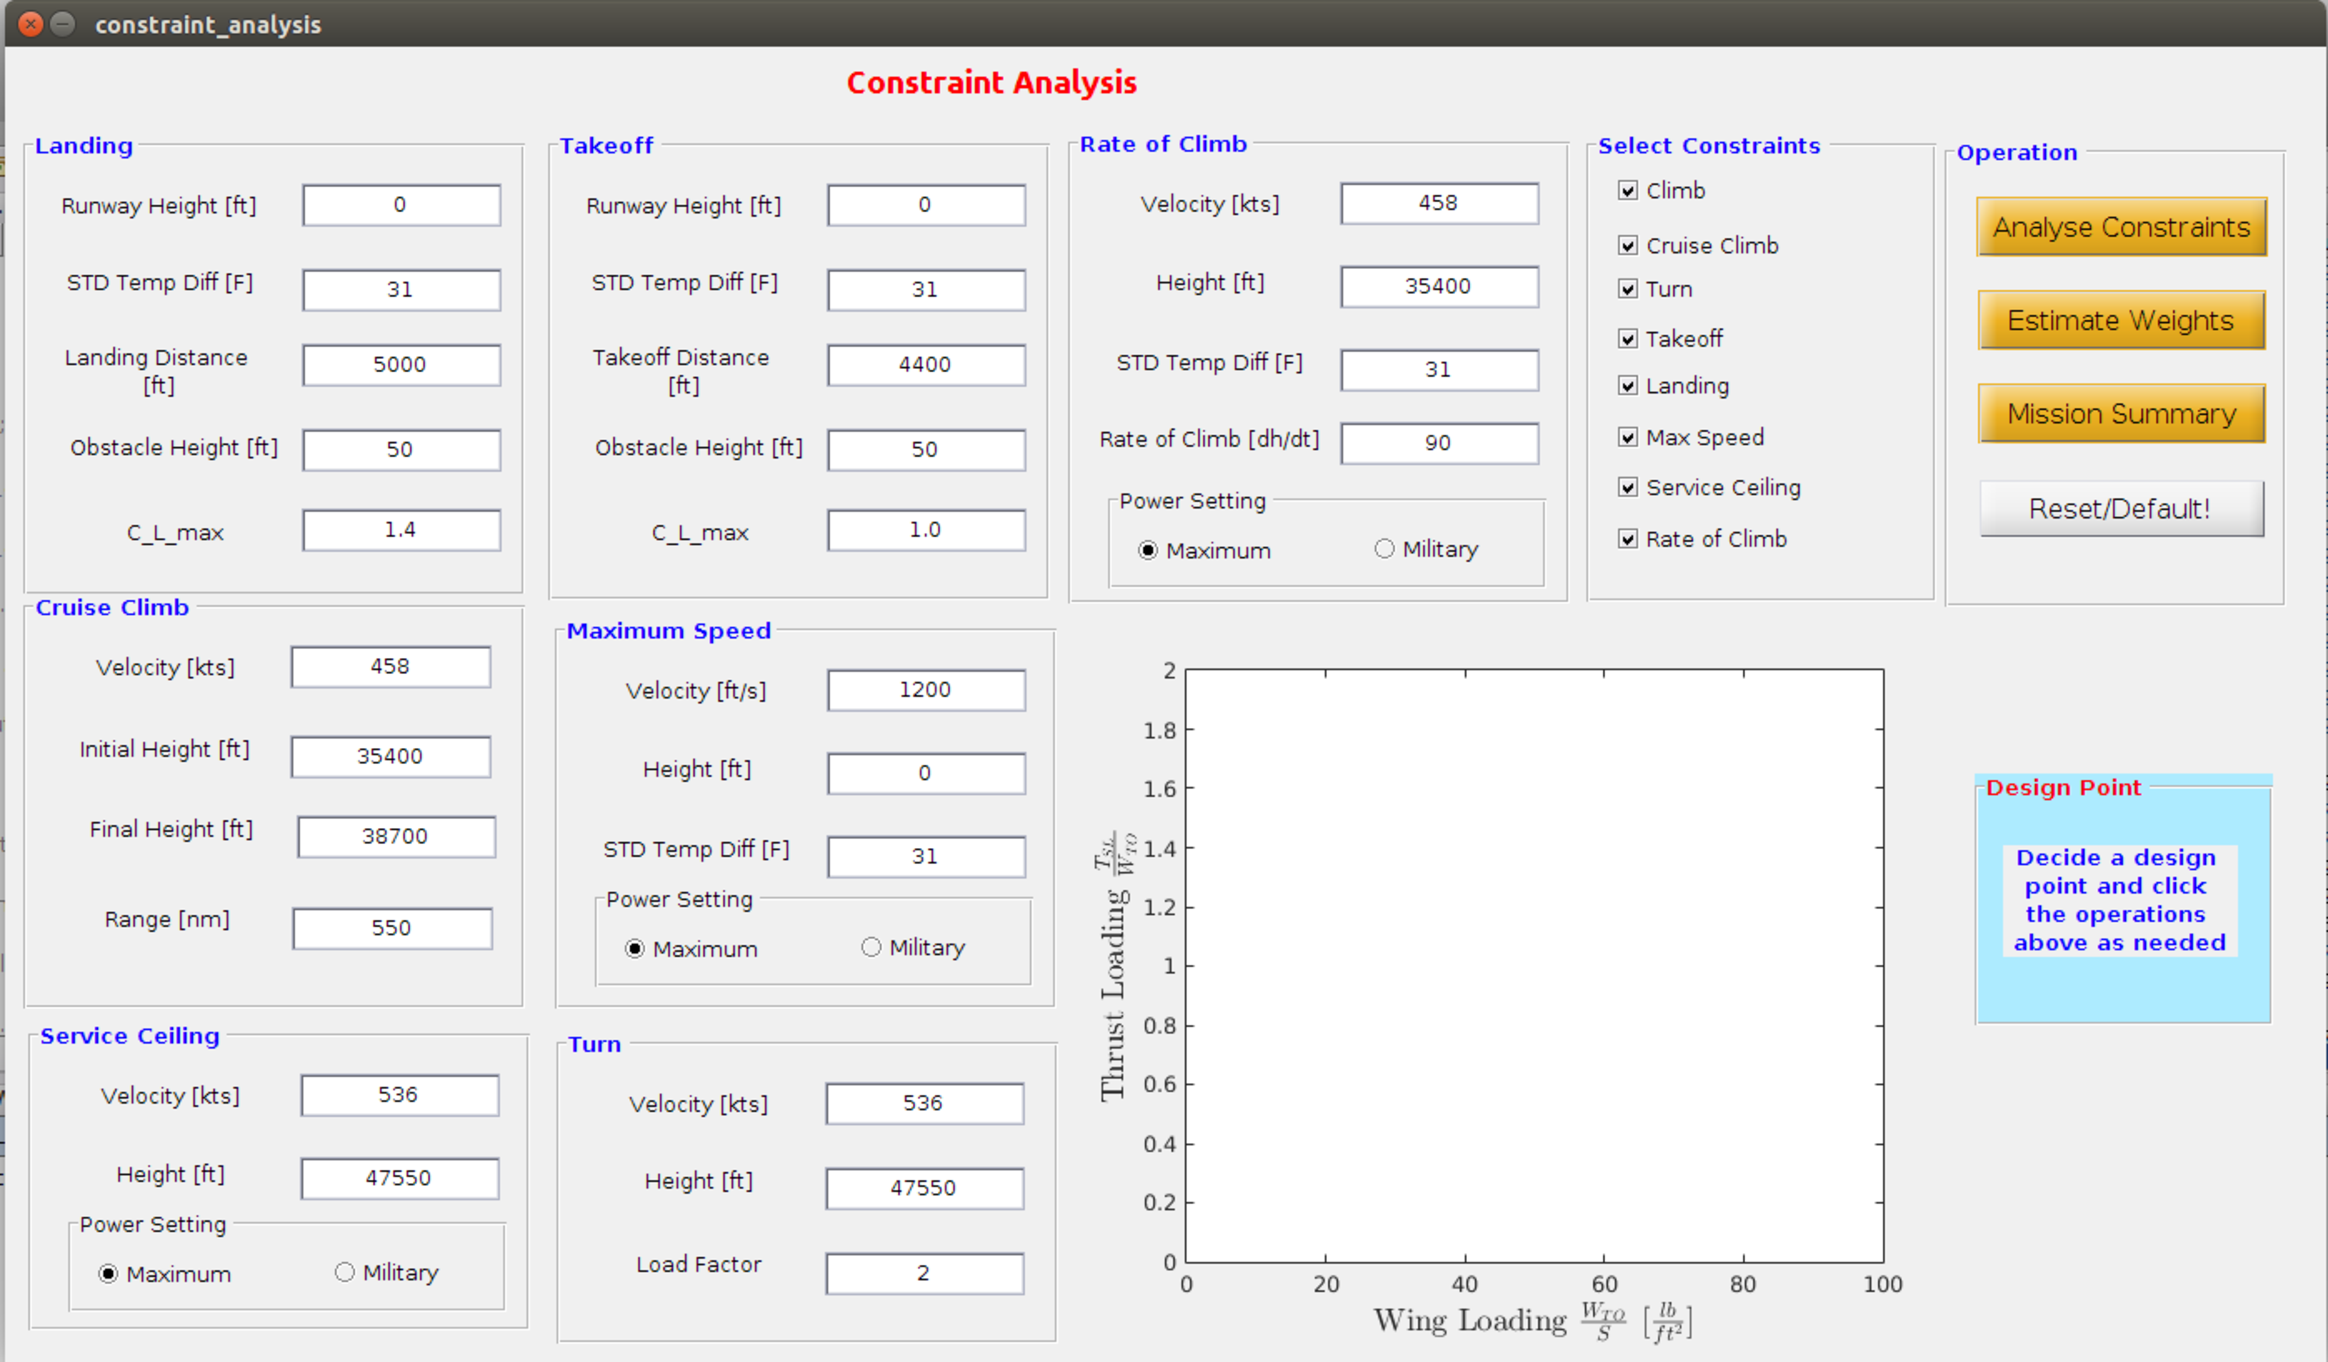
\includegraphics[scale=0.45]{figures/constraints_layout.pdf}
	\caption{Figure showing the constraint analysis layout.}
	\label{constraints_layout}
\end{figure}

\paragraph{Input:} The general inputs are velocity, height, range, thrust setting, rate of climb etc. These general inputs are assembled across different segments of mission and for different performance requirements for analysis. The constraint analyses automatically computes the fuel-burn correction factor (using Mach number, height, temperature), $\beta$, and the thrust lapse factor, $\alpha$ (using ``internal'' mission analyses). This accommodates the effects of the coupling of the \textit{Constraint Analysis} with that of \text{Weight Estimation} shown in Figure~\ref{fig:sizing_overview}.

\paragraph{Output:} 
 The  TASS provides a constraint analysis plot and enables the user to directly identify a design point in terms of thrust to weight ratio and wing loading. For further analyses, the user can now the click appropriate buttons: \textit{Estimate Weights} and \textit{Mission Summary}. Note that the \texttt{Mission Summary} needs the results of  \texttt{Estimate Weights} and therefore should be the last operation to perform.



\subsection{Weight Analysis Layout}
This layout (see Figure~\ref{weight_layout}) provides a mission weight analysis for the sizing of the system indicating the converged estimated gross takeoff weight and weight contributions from the different weight groups such as payload, fuel and crew.
\begin{figure}[h!]
	\centering
	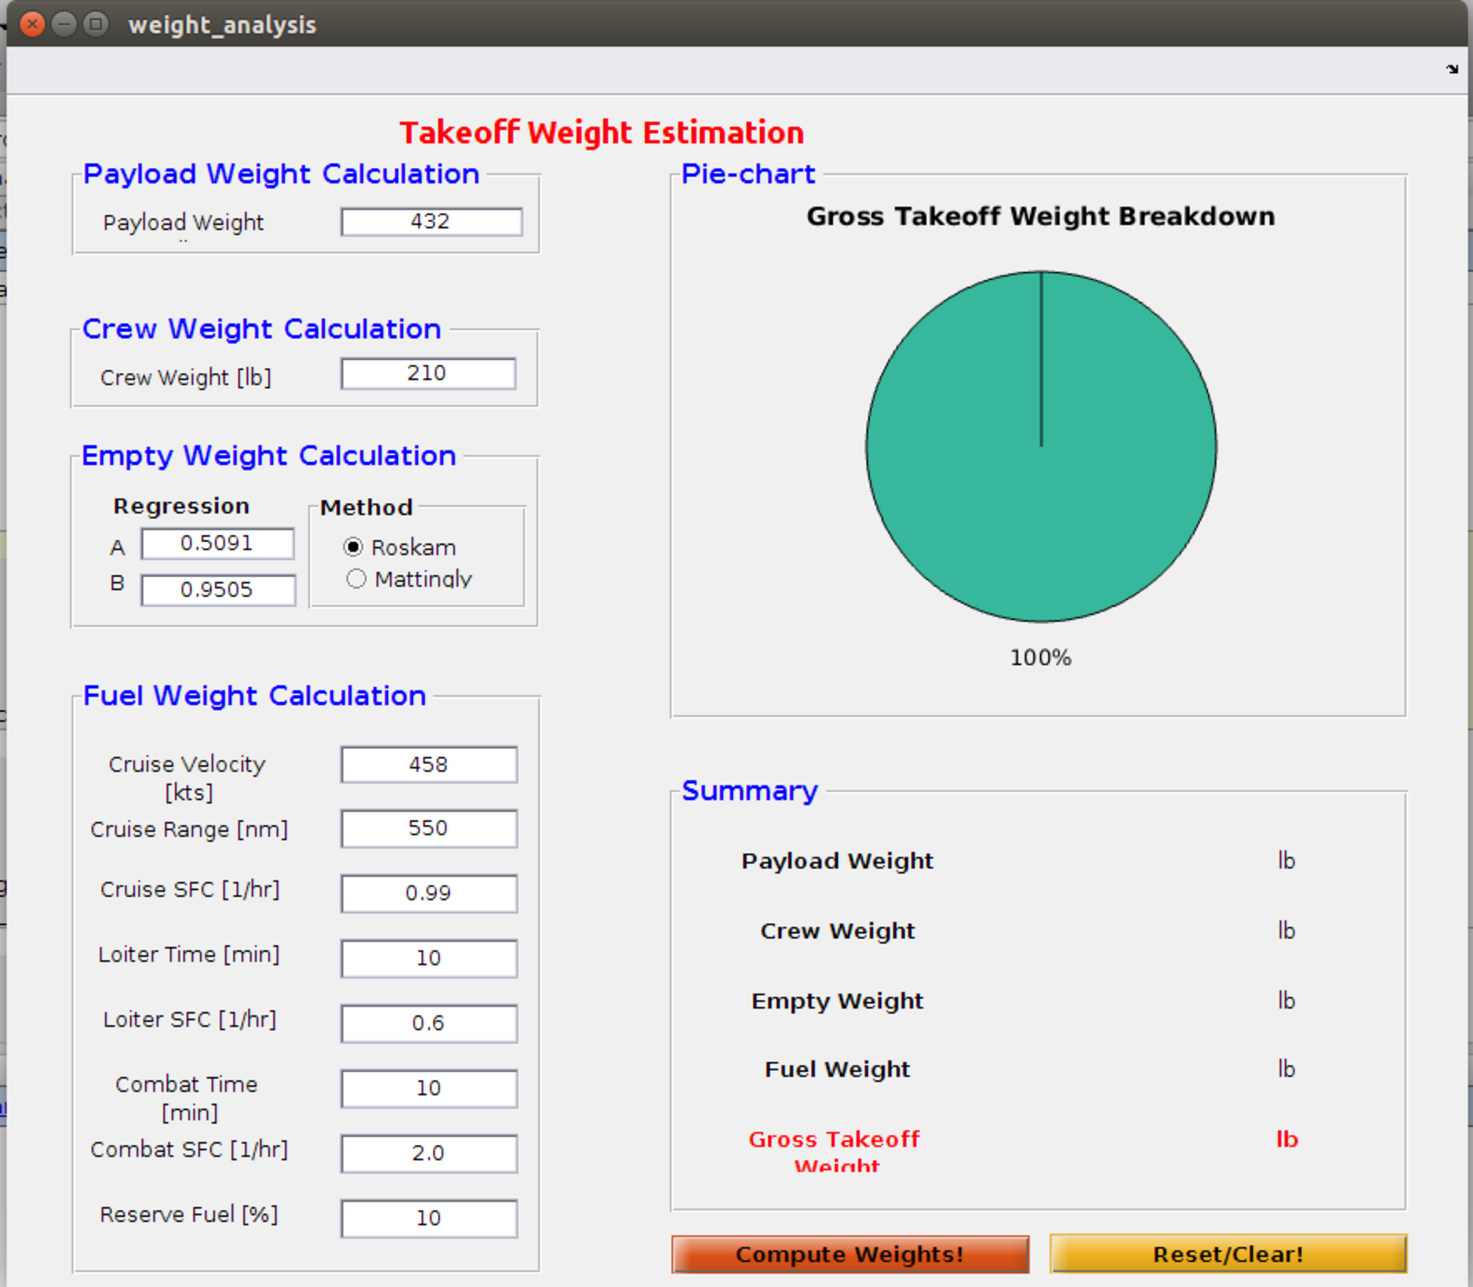
\includegraphics[scale=0.60]{figures/weight_layout.pdf}
	\caption{Figure showing the weight estimation layout.}
	\label{weight_layout}
\end{figure}
\paragraph{Execution:} This layout can be executed by typing \texttt{weight\_analysis} in MATLAB command line or by clicking the \texttt{weight\_analysis.fig} file. Alternatively, it can be executed by clicking the \texttt{Estimate Weights} button in \textit{Constraint Analysis} layout.
\paragraph{Input:}The user supplies known information such as  crew and payload weights, information about mission such as the velocity, range, loiter time and reserve fuel required. The user can experiment with nominal perturbations of these values for detailed studies.
\paragraph{Output:}
\begin{itemize}
\item  a pie-chart which represents the weight fractions (weights) as percentages of total weight
\item a table listing out the converged results of weight estimation. 
\end{itemize}

\subsection{Mission Summary Layout}
Figure~\ref{mission_layout} shows the layout designed for producing the summary of the mission in terms of different segments identified in Table~\ref{tab:requirements}. 
\paragraph{Execution:}
There are two ways to run this layout:
\begin{itemize}
\item by typing \texttt{mission\_summary} in the MATLAB command line or by opening \texttt{mission\_summary.fig} file
\item by clicking \texttt{Mission Summary} button from \textit{constraint analysis} layout
\end{itemize}
\paragraph{Input:}
The user will supply the design point which is selected from the \textit{constraint analysis} layout and click the \texttt{Generate Summary} button.
\paragraph{Output:}
The layout will then automatically generate the following results:
\begin{itemize}
\item drag-polar plots for two representative velocities $100~ft/s$ and $1200~ft/s$
\item table containing the breakdown of performance related quantities such as $\beta$, $\frac{W_{n-1}}{W_n}$, the weight of fuel burnt, variation of gross take off weight, wing loading and thrust loading, with respect to different mission-segments

\item a text box displaying the wing planform area $S$
\end{itemize}
\begin{figure}[h!]
	\centering
	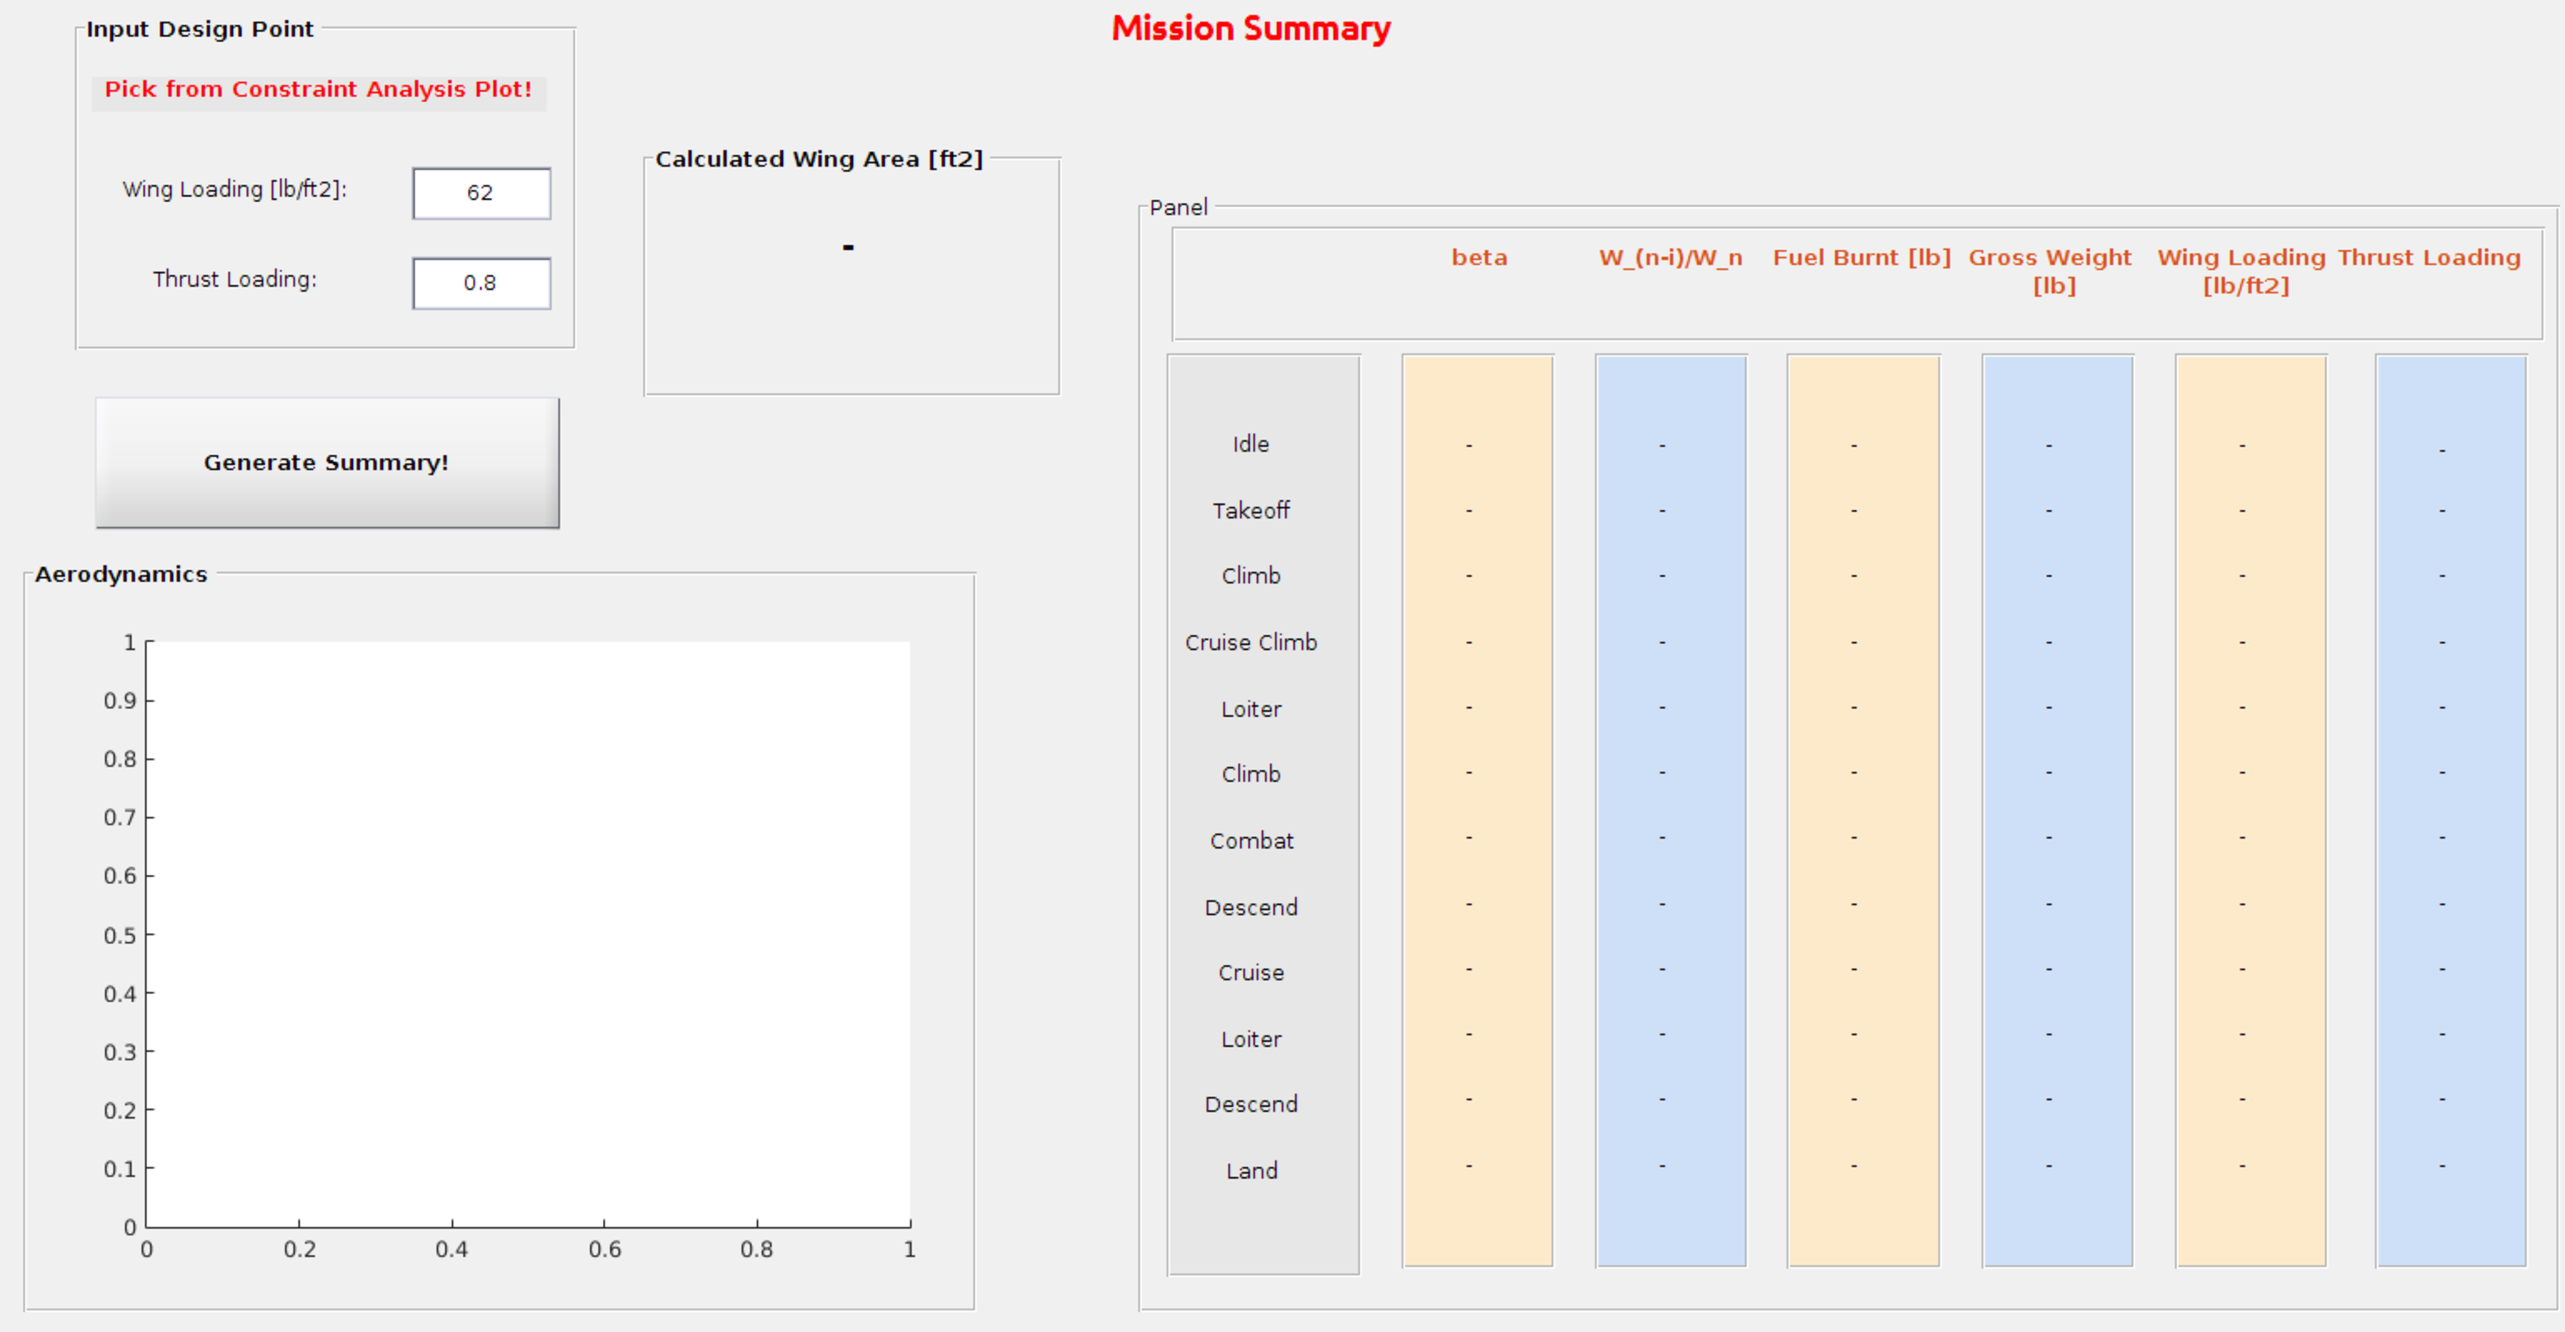
\includegraphics[scale=0.40]{figures/mission_layout.pdf}
	\caption{Figure showing the mission summary layout.}
	\label{mission_layout}
\end{figure}
\subsection{Theory and Models}\label{theory}
A rough outline of the theory, physical and mathematical models used in TASS follows. A rather comprehensive discussion on these topics can be found in the literature\cite{MattinglyText,NicolaiText,FieldingText,HoweText,RaymerText}. Figure~\ref{fig:sizing_overview} provides a generic overview of the elements involved in the sizing and synthesis process. As it can be seen, \emph{constraint analyses} and \emph{weight estimations} are pivotal in producing the design.
\begin{figure}[h!]
	\centering
	\includegraphics[scale=0.85]{figures/sizing_overview.pdf}
	\caption{A top level overview of sizing and synthesis process implemented in TASS\cite{MavrisNotes}.}
	\label{fig:sizing_overview}
\end{figure}

\paragraph{Standard Atmosphere Model:}~The toolkit automatically computes the standard atmosphere conditions based on the U.S. Standard Atmosphere model\cite{US,sky}.  The standard atmosphere model provides the temperature, speed of sound (Mach number), pressure and density as a function of height in the calculations.

\paragraph{Mattingly Energy Equation:} The performance constraints and requirements are set as functions of \emph{thrust loading} (thrust-to-weight ratio) and \emph{wing loading}, the two sizing parameters that contain key information about the top level characteristics of the system\cite{MattinglyText}. The Mattingly Master Enerygy equation is:
\beq\label{eq:energy}
\dfrac{T_{SL}}{W_{TO}} = \dfrac{\beta}{\alpha} 
\left\{ \dfrac{qS}{\beta W_{TO}}
\left[ K_1
\left(
      \dfrac{n\beta W_{TO}}{qS}
\right)^2 
+
K_2
\left(
  \dfrac{n\beta W_{TO}}{qS}
\right) +
C_{D_{0}}
+
\dfrac{R}{qS}
\right]
+
\dfrac{1}{V} \dfrac{d}{dt} \left( h + \dfrac{V^2}{2g_0}\right)
\right\}
\eeq
Table~\ref{tab:param_energy} contains a short definition of the parameters in Eq.~\ref{eq:energy}. 
\begin{table}[h]
\caption{Parameters in Mattingly Energy Equation}
%\medskip
\centering 
\begin{tabular}{c c c c}
\hline\hline
 {Parameter} & Description & English Unit \\
\hline\hline
$T_{SL}$  & sea-level thrust           & lb  \\
$W_{TO}$  & take-off gross weight      & lb   \\
$q$      & dynamic pressure           & $lb/ft^2$ \\
$S$      & wing planform area         & $ft^2$   \\
$C_{D_0}$ & drag at zero lift          &  no unit \\
$K_1$    &  Parasitic Drag constant   &   no unit       \\ 
$K_2$    & Interference drag          &   no unit      \\
$q$      & load factor                & no unit \\ 
$R$      &  Resistance Drag           &  $lb$     \\ 
$V$      &  velocity(speed)           &  $ft/s$  \\
$h$     &  altitude from sea level   & $ft$    \\
$g_0$   &  gravity at sea level      & $ft/s^2$ \\
$\alpha$&  thrust lapse correction   &  no unit  \\
$\beta$ & fuel burn correction       &    no unit\\
\hline
\end{tabular}
\label{tab:param_energy}
\end{table}

%%%%

\section{Fighter Aircraft Design}
This section describes the results of the aircraft designed using TASS in response to the mission and requirements are outlined in RFP\cite{MavrisNotes}. After the discussion of individual results, the design produced by the TASS will be compared to the design of the actual aircraft.

\subsection{Aircraft Requirements}\label{requirements}
 The conceptual design process begins with a defined set of requirements. These requirements lay-out specific constraints and design goals that the end-system must be capable of achieving.  These goals and constraints are often presented the form of Request for Proposal (RFP). %RFP for the fighter is given in Appendix~\ref{}. 
\paragraph{Mission Profile:}
Table~\ref{tab:requirements} breaks-down the performance requirements of the aircraft to be designed using the TASS. 
\begin{table}[h]
\caption{Requirements of the fighter aircraft and for different stages in the mission profile}
\centering 
\begin{tabular}{c| c| c}
\hline\hline
{Segment} & Phase       & Performance Requirements \\
\hline\hline
0-1 	& Takeoff 	& Distance $4400~ft$ \\
	&		& Clear obstacle at $50~ft$\\
	& 		& Maximum power with afterburners\\
	&		& Sea level runway at $90~F$\\\hline
1-2	& Climb		& Altitude 35400~ft \\
	& 		& Full military power without afterburners\\
	&		& Maximum rate of climb $90~ft/s$\\
\hline
2-3 	& Cruise climb	& Altitude 38700~ft \\
	&		& Distance 550 nautical miles \\
	&		& Cruise speed 458 knots\\
	&		& Normal power \\
\hline
3-4 	& Loiter	& Altitude 38700 ft\\
	&		& 10 minutes loiter \\
	& 		& normal power\\
\hline
4-5	& Climb		& Altitude 47550 ft\\
\hline
5-6	& Combat 	& Maximum power with afterburners \\
	&		& Duration 5 minutes \\
	& 		& Speed 536 knots \\
\hline
6-7	& Descend 	& Descend to 37000 ft\\
\hline
7-8	& Cruise 	& Altitude 37000 ft\\
	& 		& Distance 550 nautical miles\\
	&		& Normal power\\
\hline
8-9	& Loiter	& 10 minutes  \\	
	& 		& Altitude 35000 ft\\
	&		& Maximum endurance conditions \\
\hline
9-10	& Descend 	& Descend and line up for landing\\
\hline
10-11	& Landing	& Distance 5000 ft \\
	&		& Without highilift devices\\	
	&		& 10$\%$ fuel reserve\\
\hline\hline
\end{tabular}
\label{tab:requirements}
\end{table}
\paragraph{Functional Requirements:}
The functional requirement of the aircraft is to carryout a military mission, which is:
\begin{itemize}
\item to carry a crew member weighing  $210~lbs$ 
\item to carry a payload of $432~lb$
\end{itemize}
\paragraph{Performance Requirements:}
The elemets in mission profile are decomposed into performance requirements that are tabulated in Table~\ref{tab:performance_reqs}.
\begin{table}[h!]
\caption{Performance requirements of the desired aircraft}
\centering 
\begin{tabular}{c | c}
\hline\hline
Item  & Performance Requirements \\
\hline\hline
Takeoff distance 	& $4400~ft$ at sea-level and $90F$ temperature\\
Landing distance        & $5000~ft$  at sea-level and $90F$ temperature \\
Maximum air speed       & $1200~ft/s$ at sea-level \\
Maximum rate of climb   & $90~ft/s$\\
Manueverability at Peak Altitude                & 47550 ft\\
Turn                    & 2g sustained turn~\footnote{Assumed due to the nature of the mission}\\
\hline\hline
\end{tabular}
\label{tab:performance_reqs}
\end{table}
This tables gives rise to the following constraints that take part in the constraint analysis.

\subsection{Constraint Analysis}
By manipulating Eq.~\ref{eq:energy} various constraints pertaining to the mission can be derived. Detailed derivation and treatment of such constraints can be found in Mattingly~\etal\cite{MattinglyText}. TASS implemented seven constraints pertaining to the requirements.
\begin{enumerate}
\item Rate of climb constraint
\item Takeoff constraint
\item Landing constraint
\item $2g$ combat turn maneuver constraint
\item service ceiling constraint
\item maximum speed constraint
\item cruise climb constraint
\end{enumerate}
These constrains are derived from the requirements given in the previous sections. The inputs pertaining to these constraints are adopted from the requirements and nominal values given in the literature~\cite{MattinglyText}.
\paragraph{Input:}
Figure~\ref{input_con} shows the default inputs that were used for the constraint analysis. The user can use the layout for other set of inputs too.
\begin{figure}[h!]
\centering
	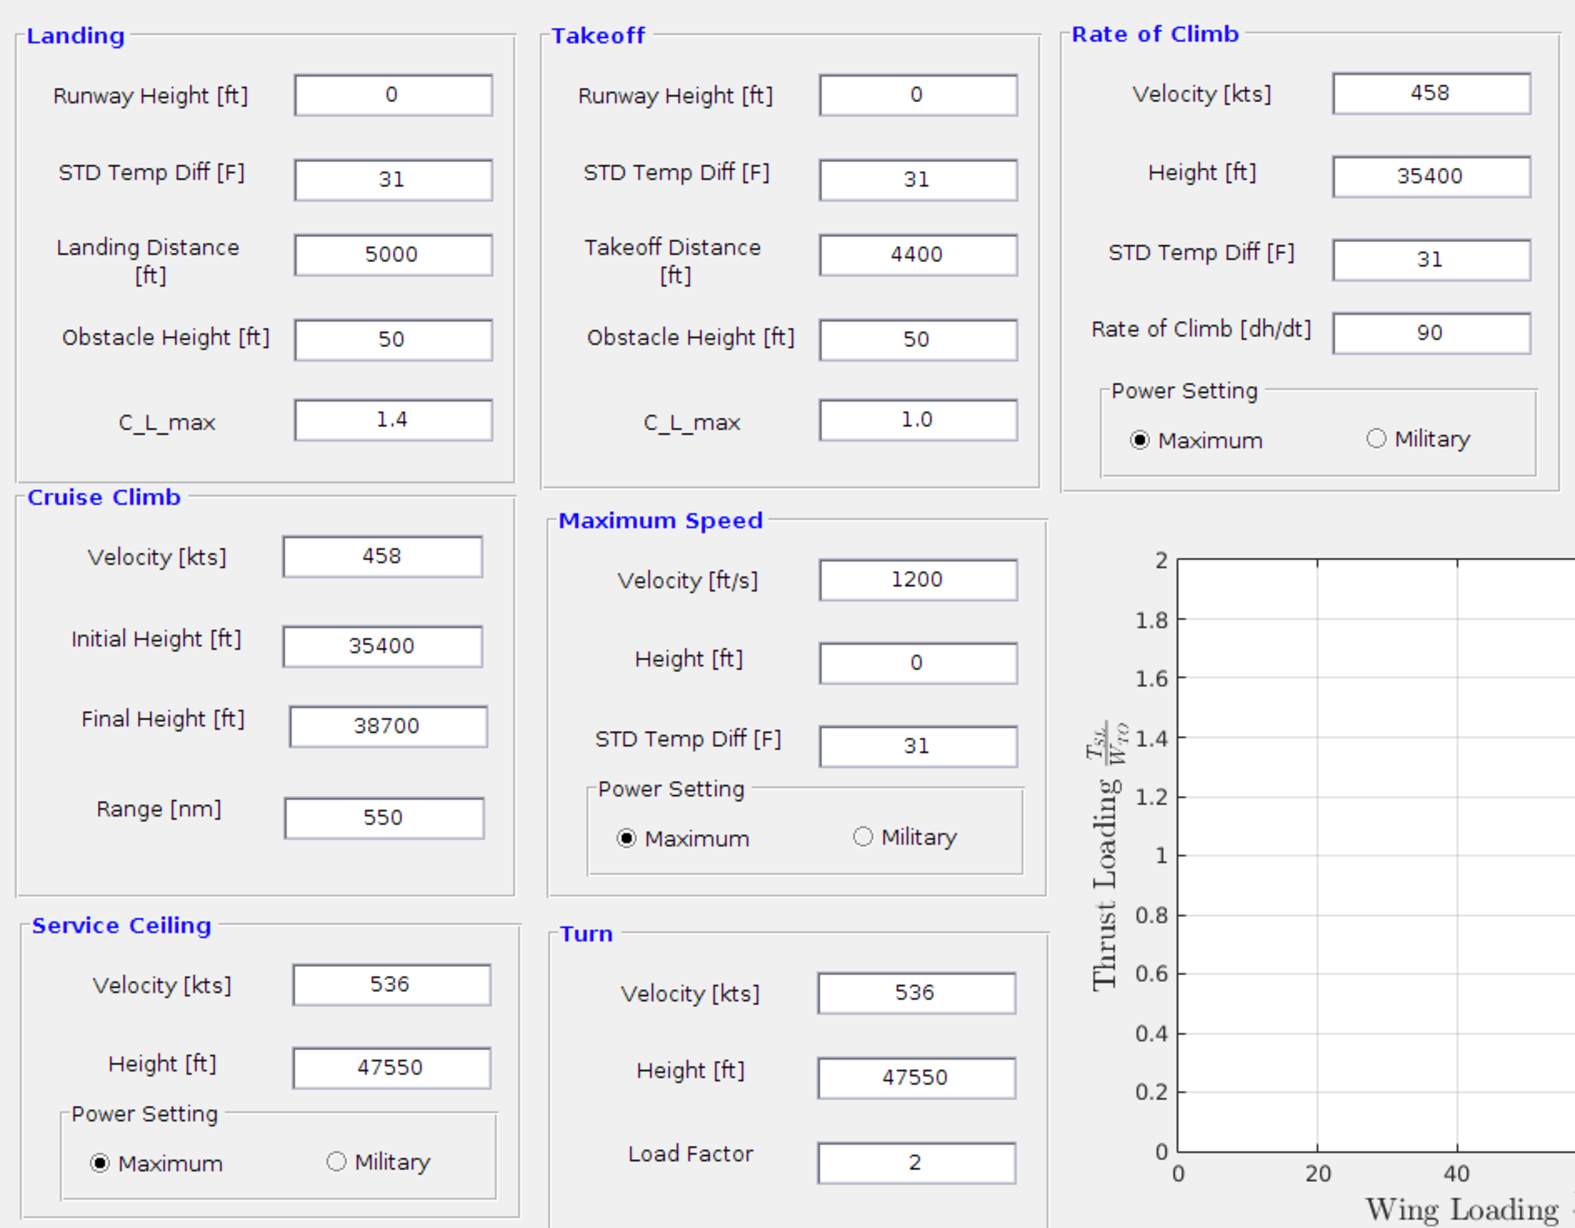
\includegraphics[scale=0.6]{figures/con_input.pdf}
        \caption{Figure showing the inputs for constraint analysis.}
\label{input_con}
\end{figure}
\begin{figure}[h!]
\centering
	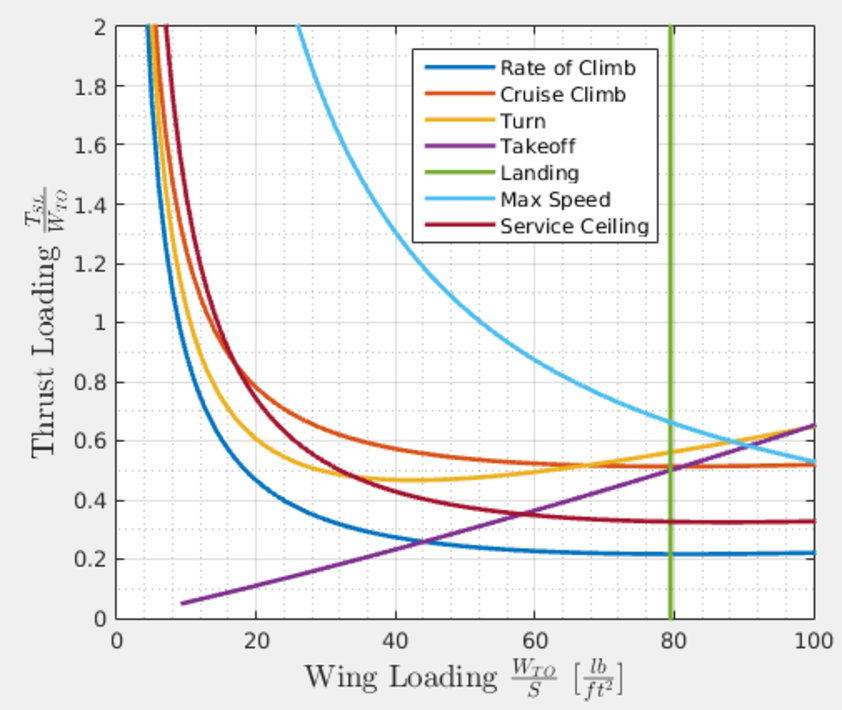
\includegraphics[scale=0.6]{figures/constraint_plot.pdf}
        \caption{Plot showing the constraints for the required design.}
\label{constraint_plot}
\end{figure}
\paragraph{Output:}
Figure~\ref{constraint_plot} shows the plot of all the seven constraints. It can be seen that the most critical constraints that drive the design are $(a)$ the $1200~ft$ maximum speed requirement at sea-level and $(b)$ the landing in a $5000~ft$ runway past a $50~ft$ obstacle. This yields the feasible design space as the ones that are between these two constraints. A simple perturbation of load factor as 3 gives the constraint plot shown in Figure~\ref{load}. Similar perturbations can be carried out for detailed analysis but such a scope is not explored in this document.
\begin{figure}[h!]
\centering
	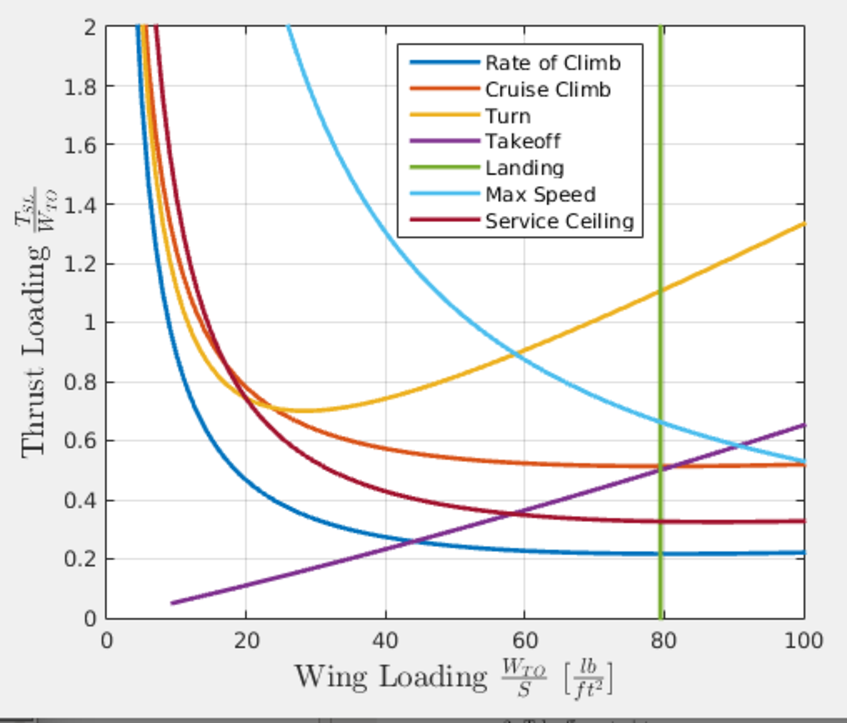
\includegraphics[scale=0.6]{figures/load3.pdf}
        \caption{Plot showing standard constraints along with load factor $n=3$.}
\label{load}
\end{figure}

\subsection{Weight Estimation}
The  takeoff gross weight $W_{TO}$ can be estimated using
\beq\label{eq:takeoff_weight}
W_{TO} = W_C + W_P +W_E +W_F
\eeq
where $W_C$ is the crew weight, $W_P$ is the payload weight, $W_E$ is the empty weight and $W_F$ is the fuel weight.
\paragraph{Payload and Crew Weights:}~ The design is done to carry a crew member who weighs $210~lbs$ and  a payload of $432~lbs$. Though this is an expendable payload as per the requirement which is dropped-off at some point in the mission, it is assumed that in the event of aborting the mission, the airplane has to carry the payload back to the base, and thus it is treated as a non-expendable payload. User input panels that facilitate the inputs of these weights is shown  in Figure~\ref{payload_crew_weight_panel}.
\begin{figure}[h!]
	\centering
	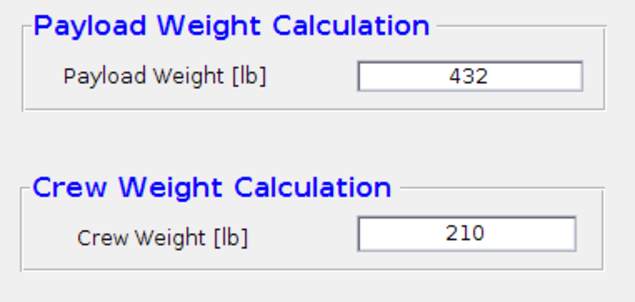
\includegraphics[scale=0.5]{figures/payload_crew_weight_panel.pdf}
	\caption{Panel designed for inputting the payload and crew weights.}
	\label{payload_crew_weight_panel}
\end{figure}

\paragraph{Empty Weight Estimation:}~It is rather difficult to estimate the empty and fuel weight compared to the other counterparts. The empty weight is found using empirical correlations of  historical data. In the toolkit both, Mattingly\cite{MattinglyText} (Eq. 3.52) and Roskam\cite{RoskamText} text based models are implemented and the user has the flexibility to choose between the two. The user only needs to input the regression constants $A$ and $B$ in the \texttt{weight analysis layout}, under \textit{empty weight panel}. The panel uses the following default values: $A=0.5091$ and $B=0.9505$, which pertains to the current design under study and is adopted from Roskam\cite{RoskamText} (Eq. 2.16). The input panel is shown in Figure~\ref{panel_empty_weight}:
 \begin{figure}[h!]
	\centering
	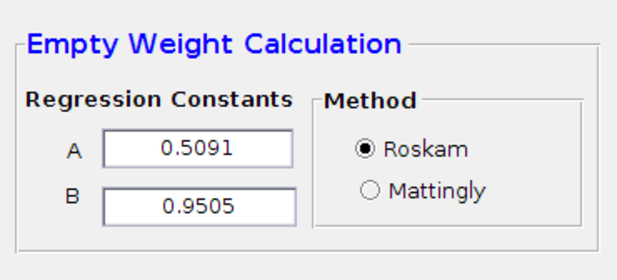
\includegraphics[scale=0.5]{figures/empty_weight_panel.pdf}
	\caption{Input panel facilitating the selection of different models for empirical estimation of empty weights.}
	\label{panel_empty_weight}
\end{figure}

\paragraph{Fuel Weight Estimation:}~Fuel consumed throughout the mission is modeled by breaking down the mission into various segments as shown in Table~\ref{tab:requirements}.
\begin{figure}[h!]
	\centering
	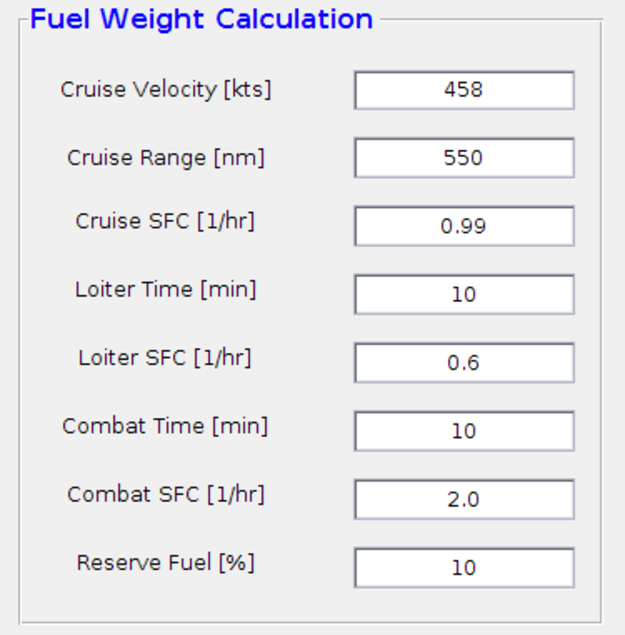
\includegraphics[scale=0.5]{figures/fuel_weight_panel.pdf}
	\caption{Input panel for fuel weight calculations.}
	\label{panel_fuel_weight}
\end{figure}
The fuel consumed during each segment is modeled based on the values provided in Raymer~\cite{RaymerText}. For the cruise segments alone, the fuel burn ordinary differential equation is integrated using the values and procedure given in Section (3.4.1) of Mattingly~\cite{MattinglyText}. The the purpose of reusability for similar missions, important inputs have been externalized in the panel, as shown in Figure~\ref{panel_fuel_weight}. The default values are the ones that are pertaining to the current mission and are assembled from RPF and sources cited above. The user can use the panel for analyzing similar configurations that follow the same mission with different values.

\paragraph{Weights Breakdown:}
At the end of the mission analysis segment-by-segment, the toolkit provides the weights breakdown in the form of a pie-chart and table (see Figure~\ref{weight_result}).
\begin{figure}[H]
\centering
	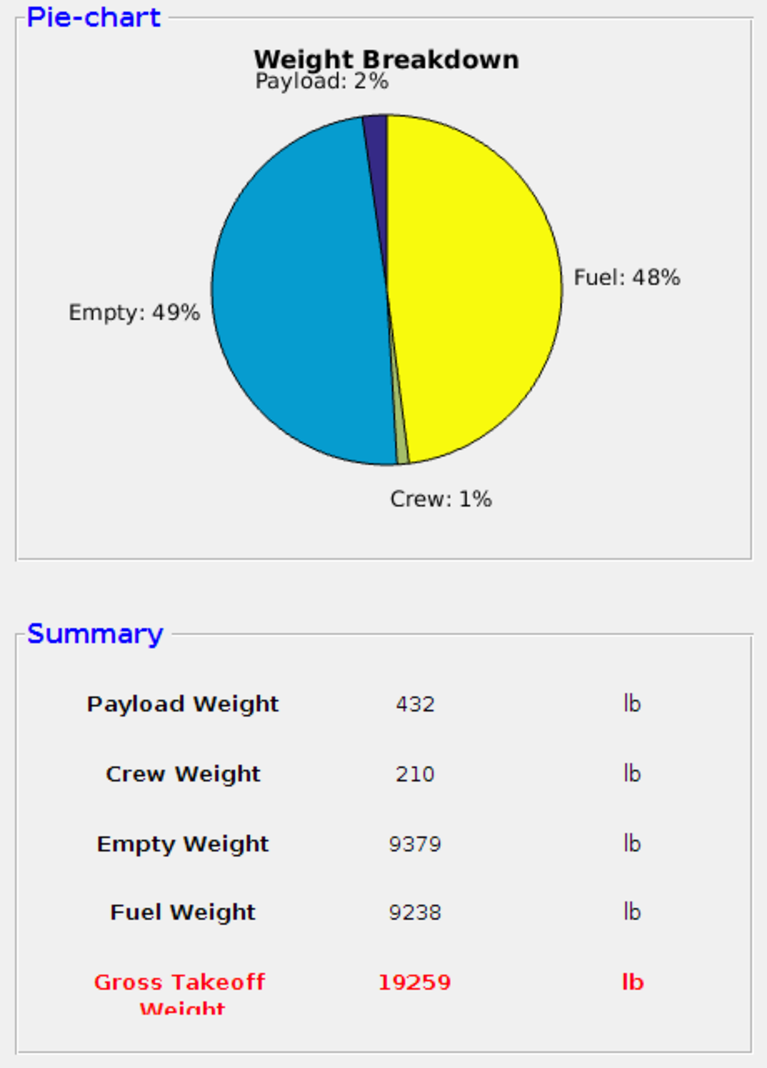
\includegraphics[scale=0.5]{figures/weight_result.pdf}
        \caption{A pie-chart showing the weight fractions (top) and the table summarizing the actual weights (bottom).}
\label{weight_result}
\end{figure}

\subsection{Mission Summary}

Finally the summary of the mission is obtained by inputting the design point to \textit{Mission Summary} layout. A complete breakdown of important parameters is shown (see Figure~\ref{missionsum}). Also a drag-polar plot is generated by this layout (see Figure~\ref{dragpolar}). The reference area is found to be $275~ft^2$.

\begin{figure}[h]
\centering
	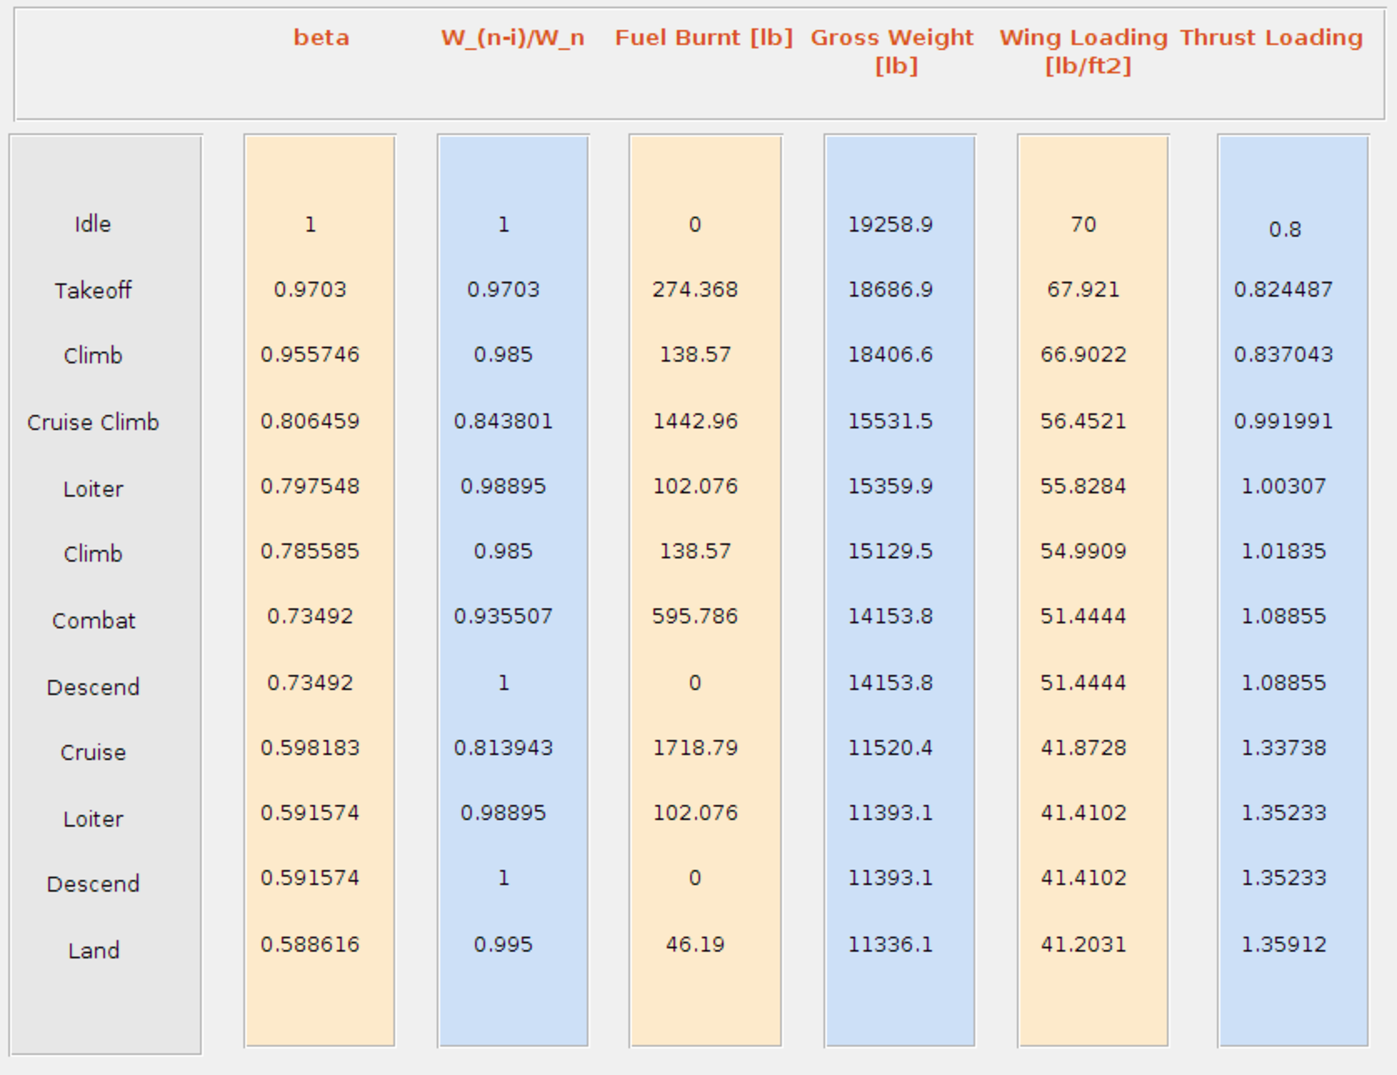
\includegraphics[scale=0.6]{figures/missionsum.pdf}
        \caption{Breakdown of mission parameters across different mission segments.}
\label{missionsum}
\end{figure}


\begin{figure}[h]
\centering
	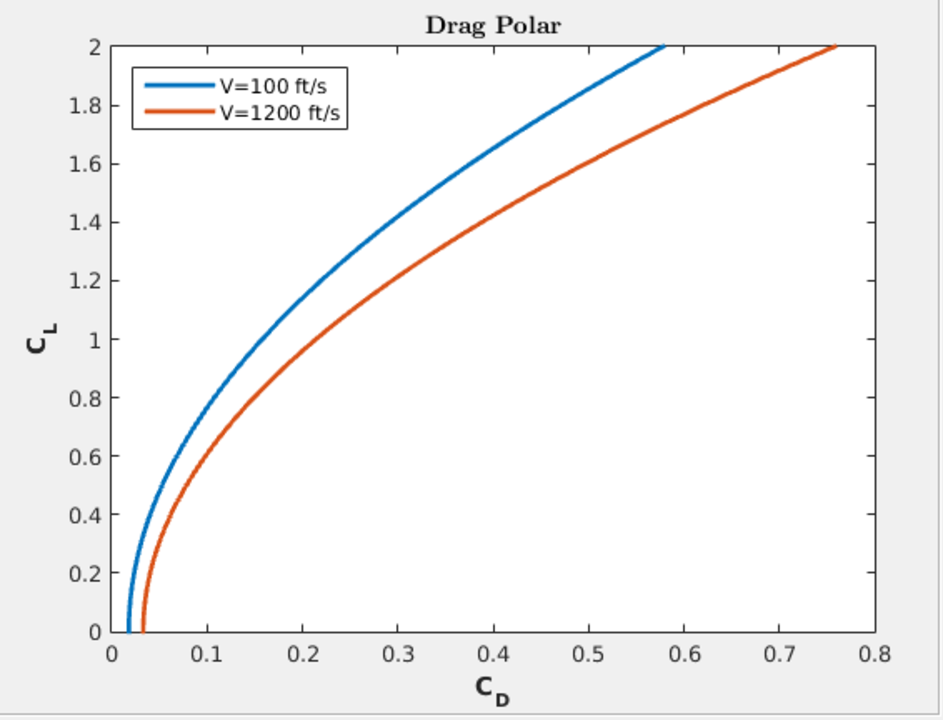
\includegraphics[scale=0.45]{figures/dragpolar.pdf}
        \caption{Plot of drag polar for two representative velocities at sea-level.}
\label{dragpolar}
\end{figure}





\subsection{Benchmarking the design}
\begin{table}[h!]
\caption{Validation of the F-86L Sabre design produced by the TASS}
\centering 
\begin{tabular}{c| c c c c}
\hline\hline
Design & Wing Loading $[lb/ft^2]$ & Thrust Loading & Gross Weight $[lb]$ & Planform Area $[ft^2]$ \\
\hline\hline
TASS             & 70 &  0.80 & 19259 & 275 \\
Actual           & 68 &  0.38 & 19975 & 290 \\
\hline\hline
\end{tabular}
\label{tab:validation}
\end{table}
The comparison of the design obtained using the tool with known configuration of the aircraft follows next. Table~\ref{tab:validation} presents the performance parameters that are calculated using the tool with that of the existing similar design~\cite{valid1,valid2}. For this benchmark F86-Sabre-D, the forerunner of F86-Sabre-L and also the  RFP data for the J47-GE-33 engine are used. An overall good agreement can be seen between the values except for the thrust loading, which is due to the maximum-speed constraint shown in the constraint plot. Perturbing this constraint (e.g. altitude of 40000 instead of sea-level, maximum speed of 1000~$ft/s$ instead of 1200~$ft/s$ will provide the user with a design that has a lower thrust loading.

\section{Conclusion}\label{conclusion}

This work presented a toolkit that performs sizing and synthesis of the aircraft configurations at the conceptual design level. The toolkit is provided with a graphical user-interface that helps non-expert users to simulate different requirements at the same time. It is validated against a known configuration of F-86 Sabrejet.

\bibliography{KomahannoVol}
\bibliographystyle{plain}	

\appendix

\section{Flexibility of the Tool}
\label{appendix:flexibility}

\subsection{Versatility of the Tool}

\begin{enumerate}

\item The Graphical User Interface (GUI) enables easy inputting of mission parameters to perform the analyses


\item The user can input any ``physically sound'' set of values as inputs to the three layouts that are the core-part of the TASS: (a) constraint analysis (b) mission analysis (c) mission summary

\item The plots and tables are co-located with the inputs to help study the effect of different parameter perturbations with ease


\item Clear/Reset push-buttons are provided in the tool that helps the user to start-off again with default values

\item TASS employs interpolations and extrapolations whenever it encounters data that are be rather difficult to supply or unavailable:

\begin{itemize}
\item it models the drag polar plots presented in Mattingly~\cite{MattinglyText} Section (2.3.1)
\item standard atmosphere model function~\cite{sky} used in the code that eliminated the need for treating them as constants at different stages in the mission
\end{itemize}

\end{enumerate}

\subsection{Challenges and Cons}

\begin{enumerate}

\item  Since it is extremely laborious to implement sanity checks on the user-supplied values, it is recommended that the users proactively consider the physical meaning of the values supplied (e.g. range, rate of climb)

\item The current version of TASS can only be used for designing airplanes that follow the ``same mission profile'' given in the RFP


\item In the \textit{constraint analysis layout}, provision has been made for picking only the constraints that the user determines to choose for analysis. Currently this facility is not-fully implemented due to time constraints!
\end{enumerate}

\end{document}

\begin{figure}[h!]
	\centering
	\includegraphics[scale=0.85]{sizing_overview.pdf}
	\caption{A top level overview of sizing and synthesis process implemented in TASS\cite{MavrisNotes}.}
	\label{fig:sizing_overview}
\end{figure}


predicted takeoff gross weight, T/W, and W/S, calculate the predicted maximum required thrust
at sea level and the predicted wing area. Compare these predicted values to the known values within the Standard Aircraft Characteristics.

\cite{MavrisNotes}
~\cite{NicolaiText}
~\cite{FieldingText}
~\cite{HoweText}
~\cite{RaymerText}
~\cite{Raymer2004}
